
\section{Methodology}

\subsection{D}




\subsection{ Data Analysis}
The data collected from the sensors will be analyzed using custom software created using vim. Graphs will be generated to compare the performance of each component.

	\subsubsection{Descriptive analysis}
	Using exploratory data analysis prior and current running status is determined 
	
	\subsection{Predictive analysis}
	Achieved by building predictive models. The required replacement parts as well as time required for maintenance can be determined.
	
	\subsection{Prescriptive analysis}
	This will provide insights on how to create desired outcomes i.e reduce load by 5\% for increased service life 
	
\subsection{System Modelling}

The predictive maintenance algorithm for motors system will be obtained from governing
equations from which a transfer function will be generated from the linearized model. The
transfer function will be used to generate a state space model for the system.
The observed sources of faults and their relative frequency. Such sources can be the core
components of the machine or its various sensors (such accelerometers and flow meters).
The process measurements through sensors. The number, type and location of sensors,
and their reliability and redundancies all will create both algorithm and comparative
model.
The sources of faults will translate to observed symptoms. Such cause-effect analysis will
require extensive processing of data from the available sensors.
Physical knowledge about the system dynamics.will result in mathematical modeling of
the system and its faults and from the insights of data. Understanding system dynamics
will involve detailed knowledge of relationships among various signals from the machinery
(such as input-output relationships among the actuators and sensors), the machine operating
range, and the nature of the measurements (for example, periodic, constant or stochastic).
The ultimate maintenance goal, such as fault recovery or development of a maintenance
schedule

\subsection{ Process chart}
From the generated models on, simulations will be performed using the different
controllers and the responses and other metrics will be plotted out for further analysis using NumPy and Pandas python libraries .
Values such as rise time, settling time and stochastic response will be observed to determine the system performance.
\begin{figure}
	\centering
	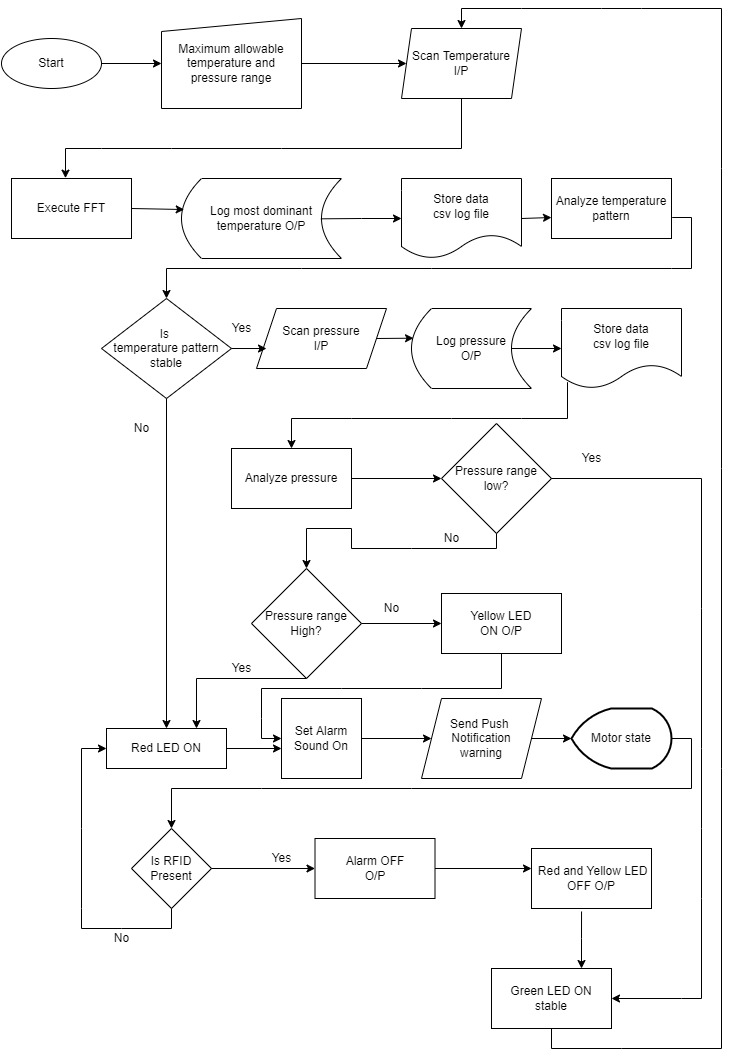
\includegraphics[width=0.7\linewidth]{Figures/model1}
	\caption{}
	\label{fig:model1}
\end{figure}


\subsection{ Sensors}
Sensors will be used to collect data from the system as it runs. These include:
\begin{enumerate}
	\item Humidity sensor
	\item Temperature sensor
	\item Flow rate sensor
	\item Pressure sensors
	\item Voltage sensor
	\item Current sensor
	
	These sensors will be used by the controller to observe system performance and optimize for each parameter.
\end{enumerate}


\subsubsection{External Force Sensor}

\subsubsection{Stewart Platform as a force sensor}
